\chapter{Detailed Report}\label{chapter:detailed_report}

\section{Tool description}
\subsection*{Chrome Cookie Extension}
\begin{itemize}
	\item \textbf{Used by}\\ Mahmoud Naser
	\item \textbf{Used for}\\ This tool was useful when inspecting cookie sessions, HTTP Headers and GET and POST variables
	\item \textbf{Useful in}\\ \vulnref{OTG-AUTHN-004} and \vulnref{OTG-AUTHN-005}
\end{itemize}

\subsection*{Acunetix Web Vulnerability Scanner}
\begin{itemize}
	\item \textbf{Used by}\\ Mahmoud Naser
	\item \textbf{Used for}\\ This tool was useful in providing a page structure to the application as well as pointing out major vulnerabilities such as Blind SQL Injection, Code execution and cross site scripting as well as other less critical errors.
	
	The disadvantage of using this tool is that the free version does not show where the vulnerability occurs as in which page it appears, and no ability to export results for later inspection.
	\item \textbf{Useful in}\\ \vulnref{OTG-INPVAL-005} and \vulnref{OTG-IDENT-002}
\end{itemize}

\subsection*{Arachni}
\begin{itemize}
	\item \textbf{Used by}\\ Florian Mauracher
	\item \textbf{Used for}\\ This tool was useful for basic application reconnaissance and identifying general issues with the application.
		As it had issues with the navigation scheme employed in our site, it was of limited utility on our site.
	\item \textbf{Useful in}\\ \vulnref{OTG-CONFIG-003} and \vulnref{OTG-INPVAL-012} and \vulnref{OTG-CRYPST-003}
\end{itemize}

\subsection*{Zed Attack Proxy}
\begin{itemize}
	\item \textbf{Used by}\\ Florian Mauracher
	\item \textbf{Used for}\\ This tool was used as a proxy to capture the complete communication between the browser and the application.
		The captured traffic was later used to identify the input vectors for the authorization section, and fuzz certain input parameters.
	\item \textbf{Useful in}\\ \vulnref{OTG-AUTHZ-001}, \vulnref{OTG-AUTHZ-002}, \vulnref{OTG-AUTHZ-003} and \vulnref{OTG-AUTHN-004}
\end{itemize}

\subsection*{SQLMap}
\begin{itemize}
	\item \textbf{Used by}\\ Alexander Lill
	\item \textbf{Used for}\\ This tool was useful for testing the different SQL attack vectors. It was used for fuzzing with different usernames and passwords and was able to retrieve the database structure, the current database user and some more internal mysql information.
	
	The disadvantage of using this tool is that it is complicated to test websites that are not simply using POST requests for the data transmission, but nested JavaScript calls.
	\item \textbf{Useful in}\\ \vulnref{OTG-INPVAL-005}
\end{itemize}

\subsection*{Skipfish}
\begin{itemize}
	\item \textbf{Used by}\\ Alexander Lill
	\item \textbf{Used for}\\ This tool was useful for finding the common vulnerabilities of the given website. This included vulnerable forms like the \texttt{/login.php}, files and directories that were referenced by the returned HTML files or which cookies were created by the website.
	
	The disadvantage of using this tool is that the results of the tool do overlap which all the other tools (e.g. arachni) but it includes less details.
	\item \textbf{Useful in}\\ \vulnref{OTG-CONFIG-003}
\end{itemize}

\subsection*{Burp Suite}
\begin{itemize}
	\item \textbf{Used by}\\ Lorenzo Donini
	\item \textbf{Used for}\\ This tool was essential for most of the tests involving an accurate analysis of the HTTP requests and responses, since it provided Proxy interception, several functionalities useful for information gathering as well as for stress testing the web applications and analyzing sessions. Additionally, Burp offers an intruder, which helped in automating most of the input validation tests (e.g. buffer overflow).
	\item \textbf{Useful in}\\ \vulnref{OTG-SESS-002}, \vulnref{OTG-SESS-003}, \vulnref{OTG-INPVAL-005}, \vulnref{OTG-INPVAL-013} and \vulnref{OTG-INPVAL-014}
\end{itemize}

\subsection*{suchsecure.py}
\begin{itemize}
	\item \textbf{Used by}\\ Lorenzo Donini
	\item \textbf{Used for}\\ This python script was useful for analyzing several bugs and business logic flaws inside the DogeBank application. This tool was custom-built for the purpose of performing specific HTTP requests to the server without having to strictly follow the business logic flow. This basic functionality also helped to flood requests and keeping a session state between operations.
	\item \textbf{Useful in}\\ \vulnref{OTG-SESS-004} and \vulnref{OTG-BUSLOGIC-001}, as well as for other bugs and business logic issues, described in chapter 4.
\end{itemize}


\clearpage
\section{Configuration and Deploy Management Testing}

%CONFIG 003
\simpleVulntitle{OTG-CONFIG-003}{Test File Extensions Handling for Sensitive Information}
\vultable{\doge}{%
	The whole configuration allows to list the content of directories and see files which should otherwise not be visible to the outside. This made analyzing the web application a lot easier.
	Also, while exploring the folder structure of the server, some leftover files were found, as well as hidden folders.
}{%
	The web application structure was brute-forced thanks to the DirBuster tool.
	Additionally, leftover files (e.g. \texttt{/employee\_registration.php~}) were found later by listing the contents of some folders, as well as other files containing sensitive information. More specifically, this is the case of the .git folder.
}{%
	Listing directories is a trivial task. Howver, in order to access the hidden .git folder an attacker must be skilled and know where to search for sensitive information.
}{%
	Having access to the data contained inside the hidden .git folder allows to get access to the whole source code of the web application, also thanks to the fact that directory listing is active.
}{%
	\cvssBaseScorePretty{N}{L}{N}{N}{U}{L}{N}{N}
}
\vultable{\gnb}{%
	Although the web application doesn't allow directory listing, it is still possible to directly open certain files. We found that some hidden folders and files containing sensitive information were left inside the folder of the web application.
}{%
	We noticed this flaw by simply observing the structure of the web application. More specifically, we found that the root folder still contained the .git folder of the project, along with a README.md file that contained the credentials to access the system as well as the database. It would also be possible to find the files contained inside the /database folder, in which the database structure as well a basic setup is stored.
}{%
	An attacker could easily brute-force the names of files and folders contained inside the root folder of the web application (perhaps using an appropriate tool). Figuring out the existence of such vulnerability is, hence, doomed to happen.
}{%
	This was the most severe vulnerability found in the GNB web application. Knowing about the existence of the .git folder doesn't help an attacker much, since directory listing is disabled (an attacker would have to brute-force the names of the objects inside of it); however, the unprotected README.md is a different matter. Once an attacker has read the credentials inside this file, he could connect to the server via ssh and get complete control over the system (root privileges included).
}{%
	\cvssBaseScorePretty{N}{L}{N}{N}{U}{H}{H}{H}
}
%CONFIG 006
\vulntitle{OTG-CONFIG-006}{Test HTTP Methods}
\vultable{\doge}{%
	We observed that the GET, POST, HEAD and OPTIONS methods are allowed. The methods PUT, DELETE and TRACE are not allowed, while other methods like COPY and MOVE are not implemented at all.
}{%
	This discovery was made using netcat.
}{%
	\na
}{%
	\na
}{%
	\secure
}
\vultable{\gnb}{%
	We observed that the GET, POST, HEAD and OPTIONS methods are allowed.	
}{%
	This discovery was made using netcat.
}{%
	\na
}{%
	\na
}{%
	\secure
}

%CONFIG 007
\vulntitle{OTG-CONFIG-007}{Test HTTP Strict Transport Security}
\vultable{\doge}{%
	The application is only accessible over HTTP.
}{%
	No HTTPS is enforced, therefore all data sent between the server and client is not encrypted.
}{%
	An attacker could perform a man in the middle attack.
}{%
	Sniffing the network traffic, all data exchanged between the server and the client can be read as clear text. No confidentiality at all is supported on this end.
}{%
	\cvssBaseScorePretty{N}{H}{N}{R}{U}{H}{H}{N}
}
\vultable{\gnb}{%
	The application is only accessible over HTTP.
}{%
	No HTTPS is enforced, therefore all data sent between the server and client is not encrypted.
}{%
	An attacker could perform a man in the middle attack.
}{%
	Sniffing the network traffic, all data exchanged between the server and the client can be read as clear text. No confidentiality at all is supported on this end.
}{%
	\cvssBaseScorePretty{N}{H}{N}{R}{U}{H}{H}{N}
}

%CONFIG 008
\vulntitle{OTG-CONFIG-008}{Test RIA cross domain policy}
\vultable{\doge}{%
	The web application doesn't support additional technologies like Flash, Silverlight or Java.
}{%
	No cross-domain policy files were found.
}{%
	\na
}{%
	\na
}{%
	\naScore
}
\vultable{\gnb}{%
	The web application doesn't support additional technologies like Flash, Silverlight or Java.
}{%
	No cross-domain policy files were found.
}{%
	\na
}{%
	\na
}{%
	\naScore
}

\clearpage
\section{Identity Management Testing}
\simpleVulntitle{OTG-IDENT-001}{Test Role Definitions}
\vultable{\doge}{%
	Clients and non-logged in users are able to access Employee privileges, see \ref{figure:RoleDefinitionsDoge}
}{%
	This was discovered through the bug searching stage and while completing the \vulnref{OTG-AUTHN-004} "Testing for bypassing authentication schema" test.
}{%
	Skill level needed to uncover this is moderate, using simple direct page access and basic trail and error with parameters is enough to exploit this bug, so the likelihood of this vulnerability is quite high 
}{%
	This could have tremendous damages to the bank, as adding employee accounts and transferring functions
}{%
	\cvssBaseScorePretty{N}{L}{N}{N}{U}{H}{H}{L}
}

\begin{figure}[h!tbp]
	\centering
	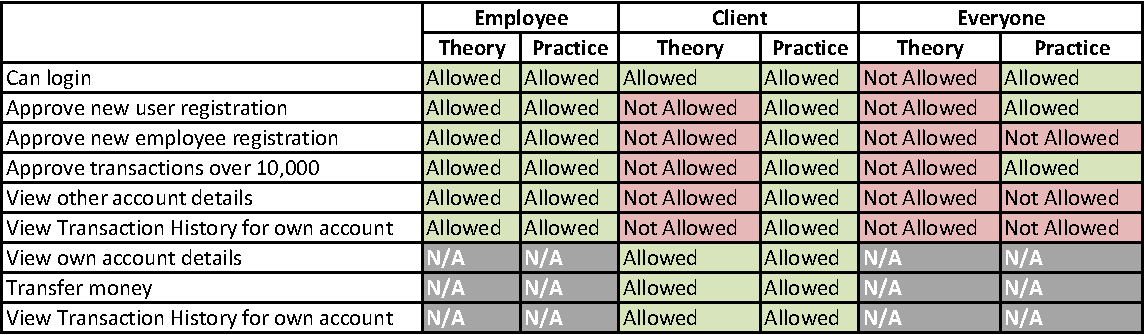
\includegraphics[width=\textwidth]{figures/RoleDefinitionsDoge}
	\caption{Role Definitions}
	\label{figure:RoleDefinitionsDoge}
\end{figure}


\vultable{\gnb}{%
	Clients, Employees and non-logged in users all act as expected, see \ref{figure:RoleDefinitionsGNB}
}{%
	This was verified through basic function testing and security testing tools (ZAP).
}{%
	\na
}{%
	\na
}{%
	\secure
}

\begin{figure}[h!tbp]
	\centering
	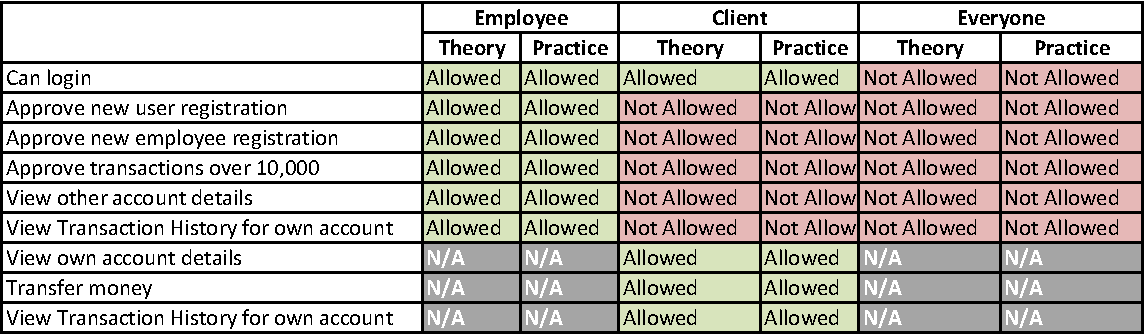
\includegraphics[width=\textwidth]{figures/RoleDefinitionsGNB}
	\caption{Role Definitions}
	\label{figure:RoleDefinitionsGNB}
\end{figure}


\vulntitle{OTG-IDENT-002}{Test User Registration Process}
\vultable{\doge}{%
	The registration process is set up for anyone to register, the process then awaits human interaction for the approval stage, this will serve an extra step of verification.

	Identities are not verified nor checked at this stage due to application limitations, email format verification is missing from the form.
	
	No CAPTCHA or similar tests available to test for human accounts
}{%
	The email verification test was discovered through trail and error while registering.
	Lack of human testing was found through simple observation.
}{%
	likely, due to intentional or unintentional mistyping.
	Robot accounts are less likely to occur and it depends on the skill level of the attacker.
}{%
	No serious impact as TAN codes are not sent to the email.
	Robot accounts can be used to perform a DOS attack. 
}{%
	\cvssBaseScorePretty{N}{L}{N}{N}{U}{N}{N}{L}
}

\vultable{\gnb}{%
	The registration process is set up for anyone to register, the process then awaits human interaction for the approval stage, this will serve an extra step of verification.
	
	Identities are not verified nor checked at this stage due to application limitations.
	
	No CAPTCHA or similar tests available to test for human accounts.
}{%
	Lack of human testing was found through simple observation.
}{%
	Robot accounts are less likely to occur and it depends on the skill level of the attacker.
}{%
	Robot accounts can be used to perform a DOS attack. 
}{%
	\cvssBaseScorePretty{N}{L}{N}{N}{U}{N}{N}{L}
}

\vulntitle{OTG-IDENT-003}{Test Account Provisioning Process}
\vultable{\doge}{%
	Provisioning clients is an easy process with no effective mechanisms to verify or vet clients besides a manual approval process.
	
	Vulnerabilities with creating the client account have been discussed in the previous section \vulnref{OTG-IDENT-002}, but using  \vulnref{OTG-AUTHZ-002} an non-authenticated user is able to approve a client user request.
	
	Provisioning Employees is set up to only be possible by other employees, but using  \vulnref{OTG-AUTHZ-001}, a non-authenticated user is able to create an employee account.
}{%
	This was discovered through trail and error in the bug discovery phase.
}{%
	This vulnerability requires some basic knowledge of the PHP pages and variable names, which can be obtained using basic testing tools, so while this vulnerability is likely to be discovered by an attacker with some basic skills.
}{%
	This presents some serious impact, as creating an employee account will give the attacker full access to the application and administrative functions such as creating accounts and approving money transfers. 
}{%
	\cvssBaseScorePretty{N}{L}{N}{N}{U}{N}{L}{N}
}

\vultable{\gnb}{%
	Provisioning clients is an easy process with no effective mechanisms to verify or vet clients besides a manual approval process, provisioning Employees is set up in a similar matter.
	
	Vulnerabilities with creating the client account have been discussed in the previous section \vulnref{OTG-IDENT-002}, the same applies to creating employee accounts, so a potential DOS attack is possible by creating robot accounts.
}{%
	This was found through following the given process for creating accounts.
}{%
	Robot accounts are less likely to occur and it depends on the skill level of the attacker.
}{%
	If the DOS attack is severe enough it could stop the application from from working.
}{%
	\cvssBaseScorePretty{N}{L}{N}{N}{U}{N}{N}{N}
}

\vulntitle{OTG-IDENT-004}{Testing for Account Enumeration and Guessable User Account}
\vultable{\doge}{%
	Errors provided from enumerating through the different cases are as follows :
	\begin{itemize}
		\item Valid username with correct password : Expected result of logging in 
		\item Valid username with incorrect password : Returns "Username or Password incorrect! Please try again!"
		\item Invalid username : Returns "Username or Password incorrect! Please try again!"
	\end{itemize}
}{%
	This was found through trail and error on different combinations of credentials.
}{%
	\na
}{%
	\na
}{%
	\secure
}

\vultable{\gnb}{%
	Errors provided from enumerating through the different cases are as follows :
	\begin{itemize}
		\item Valid username with correct password: Expected result of logging in 
		\item Valid username with incorrect password: Returns "Invalid login credentials!"
		\item Invalid username : Returns "Invalid login credentials!"
	\end{itemize}
}{%
	This was found through trail and error on different combinations of credentials.
}{%
	\na
}{%
	\na
}{%
	\secure
}

\vulntitle{OTG-IDENT-005}{Testing for Weak or unenforced username policy}
\vultable{\doge}{%
	No username policy applied.
}{%
	\na
}{%
	\na
}{%
	\na
}{%
	\na
}

\vultable{\gnb}{%
	Username has to be in valid email address format.
}{%
	Through trail and error.
}{%
	\na
}{%
	\na
}{%
	\secure
}

\clearpage
\section{Authentication Testing}
\simpleVulntitle{OTG-AUTHN-001}{Testing for Credentials Transported over an Encrypted Channel}
\vultable{\doge}{%
	Due to the fact, that no encryption is used when accessing the application, credentials transported over an encrypted channel are vulnerable.
		
	Relevant information regarding unencrypted communication has already been mainly covered in section \vulnref{OTG-CRYPST-003} and in \vulnref{OTG-CONFIG-007}.
}{%
	Through observation.
}{%
	Given that a simple network sniffing tracking tool would pick up the credentials, this vulnerability is likely to be exploited.
}{%
	The attacker is able access the said account, and perform actions on behalf of said user, and it the account is an employee account, the attacker would gain access to the administrative tasks
}{%
	\cvssBaseScorePretty{N}{H}{N}{R}{U}{H}{H}{N}
}

\vultable{\gnb}{%
	\same				
}{%
	\same
}{%
	\same
}{%
	\same 
}{%
	\cvssBaseScorePretty{N}{H}{N}{R}{U}{H}{H}{N}
}

\vulntitle{OTG-AUTHN-002}{Testing for default credentials}
\vultable{\doge}{%
	The Administrator had a predictable username "employee" and an easy to guess short password "pass".				
}{%
	Credentials were provided in the team report.
}{%
	If an attacker is performing a basic dictionary attack, this vulnerability would very likely be discovered. 
}{%
	Gaining access to the employee account would allow the attacker to perform administrative tasks on the application.	
}{%
	\cvssBaseScorePretty{N}{L}{N}{N}{U}{H}{H}{L}
}

\vultable{\gnb}{%
	Administrator(Employee) and client users did not have predictable credentials.				
}{%
	Credentials were provided in the team report.
}{%
	\na 
}{%
	\na
}{%
	\secure
}

\vulntitle{OTG-AUTHN-003}{Testing for Weak lock out mechanism}
\vultable{\doge}{%
	No lockout mechanism is deployed. 
}{%
	Through trail and error.
}{%
	This allows for brute force attacks on accounts if the attacker has a username. 
}{%
	Gaining access to an employee or client account, which allow the attacker to perform that accounts tasks.	
}{%
	\cvssBaseScorePretty{N}{L}{N}{N}{U}{L}{L}{N}
}

\vultable{\gnb}{%
	\same
}{%
	\same
}{%
	\same
}{%
	\same
}{%
	\cvssBaseScorePretty{N}{L}{N}{N}{U}{L}{L}{N}
}

\vulntitle{OTG-AUTHN-004}{Testing for bypassing authentication schema}
\vultable{\doge}{%
	Through direct page access (see \vulnref{OTG-AUTHZ-002} and \vulnref{OTG-AUTHZ-004}), and SQL injection (see \ref{over:sql}) a non-authenticated user is able to gain access to both client and employee functions without being logged in.
	
	For more details on what privileges can a non-authenticated user can exploit, please refer to \ref{figure:RoleDefinitionsDoge}.
	\begin{itemize}
	\item Direct page access example : the url \texttt{/downloadTans.php?userid=1} allows a non authorized user to download the TAN codes for the user with the user\_id of 1.
	\item SQL Injection example : by using the username 
	\textit{\rq OR 1=1 AND user\_name=`employee' \#} an attacker can gain access to the admin account `employee'
	\end{itemize}
}{%
	This was discovered through trail and error in the bug discovery phase.
}{%
	This vulnerability requires some basic knowledge of the PHP pages and variable names, which can be obtained using basic testing tools, so while this vulnerability is likely to be discovered by an attacker with some basic skills.
}{%
	This presents some serious impact, as creating an employee account will give the attacker full access to the application and administrative functions such as creating accounts and approving money transfers. 	
}{%
	\cvssBaseScorePretty{N}{L}{N}{N}{U}{H}{H}{L}
}

\vultable{\gnb}{%
	The PHP Session ID cookie variable is not destroyed after logout, and even though the user is unable to use the "back" option on the browser, the PHP Session ID does not change though making it extremely predictable after logging 
}{%
	This was done through cookie inspection using the chrome and Firefox Developer extensions.
}{%
	The skill level required for exploiting this is minimal, Knowledge needed for this attack is basic cookie inspection and injection and Network sniffing.
}{%
	Overtake an existing user session and gain access to that users privileges.
}{%
	\cvssBaseScorePretty{N}{H}{N}{R}{U}{L}{L}{L}
}

\vulntitle{OTG-AUTHN-005}{Test remember password functionality}
\vultable{\doge}{%
	Passwords in this application are sent in clear text.
}{%
	Through HTTP Header inspection
}{%
	The skill level required for exploiting this is minimal, Knowledge needed for this attack is basic HTTP Header inspection and Network sniffing.
}{%
	Gaining access to an employee or client account, which allow the attacker to perform that accounts tasks.	
}{%
	\cvssBaseScorePretty{N}{H}{N}{R}{U}{L}{L}{L}
}

\vultable{\gnb}{%
	\same				
}{%
	\same
}{%
	\same
}{%
	\same
}{%
	\cvssBaseScorePretty{N}{H}{N}{R}{U}{L}{L}{L}
}


\vulntitle{OTG-AUTHN-006}{Testing for Browser cache weakness}
\vultable{\doge}{%
	Browser Cache settings are set up correctly, so 'Back' on the browser does not work.
}{%
	Though observation.
}{%
	\na
}{%
	\na	
}{%
	\secure
}

\vultable{\gnb}{%
	\same				
}{%
	\same
}{%
	\same
}{%
	\same
}{%
	\secure
}


\vulntitle{OTG-AUTHN-007}{Testing for Weak password policy}
\vultable{\doge}{%
	No password policy is implemented.
}{%
	Though observation.
}{%
	The skill level required for exploiting a week password is minimal,  either through password cracking tools or social engineering.
}{%
	Gaining access to an employee or client account, which allow the attacker to perform that accounts tasks.	
}{%
	\cvssBaseScorePretty{N}{L}{N}{N}{U}{L}{L}{N}
}

\vultable{\gnb}{%
	\same				
}{%
	\same
}{%
	\same
}{%
	\same
}{%
	\cvssBaseScorePretty{N}{L}{N}{N}{U}{L}{L}{N}
}


%\vulntitle{OTG-AUTHN-008}{Testing for Weak security question/answer}
%\vulntitle{OTG-AUTHN-009}{Testing for weak password change or reset functionalities}
%\vulntitle{OTG-AUTHN-010}{Testing for Weaker authentication in alternative channel}

\clearpage
\section{Authorization Testing}

\simpleVulntitle{OTG-AUTHZ-001}{Testing Directory traversal/file include}
\vultable{\doge}{%
	No user defined input vectors to include additional files were discovered during testing.
}{%
	After capturing the requests and responses of all pages available in the application with Zed Attack proxy, the recorded traffic was checked for possible input vectors.
	No input vectors referencing files were found.
}{%
	\na
}{%
	\na
}{%
	\na
}
\vultable{\gnb}{%
	User defined input vectors were observed on all pages of the application which require authentication.
	These input vectors don't seem to be direct references to files in the web application, thus an indirect mapping of the specified names to included files is assumed.
	Due to this indirect mapping accessing arbitrary files on the server is not possible by modifying these input vectors.
	Nevertheless an authenticated attacker is able to use this mechanism to get access to all included pages as described in \vulnref{OTG-AUTHZ-002}
}{%
	After capturing the requests and responses of all pages available in the application with Zed Attack proxy, the recorded traffic was checked for possible input vectors.
	Multiple input vectors referencing sections of the site were identified, but manual testing revealed that none of these referred to filenames directly.
}{%
	\na
}{%
	\na
}{%
	\secure
}

\vulntitle{OTG-AUTHZ-002}{Testing for bypassing authorization schema}
\vultable{\doge}{%
	All employee pages are fully accessible for any authenticated user e.g. client.
}{%
	Manually accessing the address of the employee pages while being logged in as user allowed full access to these sites.
	\texttt{/employee\_home.php}
}{%
	To exploit this vulnerability an attacker needs to be aware of the address of the employee pages and have an valid client account.
}{%
	This vulnerability allows bypassing all authorization mechanisms put in place, granting the attacker the highest privileges available in the application.
}{%
	\cvssBaseScorePretty{N}{L}{L}{N}{U}{H}{H}{H}
}
\vultable{\gnb}{%
	Direct access to the employee page is not possible as client.
	However by using the file inclusion technique described in \vulnref{OTG-AUTHZ-001} an authenticated attacker is able to access all included pages of the application.
}{%
	Manual testing direct access to the employee pages (\texttt{/employee/employee.php}) did not grant any positive results.\newline
	Using the information gathered in \vulnref{OTG-AUTHZ-001} it was possible to access the employee pages by modifying the POST parameters of the client page to reference the employee pages.
	Page: \texttt{/client/client.php}\newline
	Original POST parameters:\newline
	\texttt{section=my\_accounts\&frame=account\_overview\&account=10000002}\newline
	Updated POST parameters:\newline
	\texttt{section=employee\_area\&frame=manage\_registration}\newline
	This opened the page with pending registrations which should only be visible as employee.
	Additional effort is required to start any further actions from this page (e.g.\ approving users) as the required javascript is missing and all references lead to the wrong page.
	The same applies for all other employee pages.
}{%
	To access these sites an attacker has to be authenticated and aware of the names of the employee pages.
	As the client area pages doesn't contain the required javascript code for the employee area, additional knowledge and effort is required to perform actions on the pages accessed by this method.
}{%
	This vulnerability allows bypassing all authorization mechanisms put in place, granting the attacker the highest privileges available in the application.
}{%
	\cvssBaseScorePretty{N}{H}{L}{N}{U}{H}{H}{H}
}

%\vulntitle{OTG-AUTHZ-003}{Testing for Privilege Escalation}
\vulntitle{OTG-AUTHZ-004}{Testing for Insecure Direct Object References}
\vultable{\doge}{%
	None of the direct object references that were observed in the application appears to have additional authorization or authentication checks.
}{%
	After capturing the requests and responses of all pages available in the application with Zed Attack proxy, the recorded traffic was checked for direct references to objects supplied by the user.
	Manual testing of these revealed that no authorization or authentication was in place when accessing these objects.
	\begin{itemize}
		\item Download transaction history of an arbitrary user\newline\texttt{/downloadTransaction.php?userid=1}
		\item Download tans of an arbitrary user\newline\texttt{/downloadTans.php?userid=1}
		\item Approve an arbitrary transaction without being logged in\newline\texttt{/approvetransaction.php?transid=2}
		\item Approve an arbitrary user who just registered\newline\texttt{/approveuser.php?userid=2}
	\end{itemize}
}{%
	To exploit this vulnerability an attacker needs to know the address of the pages containing the direct object references.
	The sequentially increasing user IDs starting with 1 make it easy to obtain this information for all users of the bank.
}{%
	Trough this vulnerability it is possible to directly access all functionality an employee has available.
	As this is possible even for an unauthenticated user this vulnerability is also referenced in \vulnref{OTG-AUTHN-004}.
}{%
	\cvssBaseScorePretty{N}{L}{N}{N}{U}{H}{H}{L}
}
\vultable{\gnb}{%
	No direct object references were observed.
}{%
	\na
}{%
	\na
}{%
	\na
}{%
	\secure
}

\clearpage
\section{Session Management Testing}
%SESSION 001
\simpleVulntitle{OTG-SESS-001}{Testing for Bypassing Session Management Schema}
\vultable{\doge}{%
	When accessing the application, a randomly generated PHPSESSID session cookie is set. The cookie doesn't have an expiration date nor is it tagged as secure. Apparently the session cookie is already set before logging into the application. This cookie is simply replaced by a new one once the user logs out of the application. No other cookies are set. Also if the cookie is tampered with, the server automatically generates a new cookie, containing a new session ID.
}{%
	The PHPSESSID cookie has been discovered while intercepting HTTP requests/responses using Burp. The same cookie details were later on confirmed using the Cookies plugin for browser.
}{%
	\na
}{%
	Since the only used cookie only contains the session ID, even though it is easy to change the value of the cookie, no other session values are exposed to the user. It is still possible to hijack another session by changing the entire value of the cookie with the one associated to another user (see \vulnref{OTG-SESS-004}).
}{%
	\na
}
\vultable{\gnb}{%
	The same observations made for the DogeBank application apply.
}{%
	The PHPSESSID cookie was analyzed using the Cookies plugin for browser.
}{%
	\na
}{%
	\same
}{%
	\na
}
%SESSION 002
\vulntitle{OTG-SESS-002}{Testing for Cookies attributes}
\vultable{\doge}{%
	We found that the cookie generated by the application does NOT set the following attributes:
	\begin{itemize}
		\item Secure
		\item HttpOnly
		\item Expires
	\end{itemize}
	The application also sets the domain attribute very loosely, since the path is set to the root directory "/".
}{%
	The attributes were analyzed using the Cookies plugin for browser.
}{%
	It is easy to access the cookies from Javascript, as long as the browser supports client-side scripting.
}{%
	Weak protection for cookies means that these can be accessed via Javascript to perform XSS attacks.
}{%
	\cvssBaseScorePretty{N}{H}{N}{R}{U}{L}{L}{L}
}
\vultable{\gnb}{%
	The same observations made for the DogeBank application apply.
}{%
	The attributes were analyzed using the Cookies plugin for browser.
}{%
	It is easy to access the cookies from Javascript, as long as the browser supports client-side scripting.
}{%
	Weak protection for cookies means that these can be accessed via Javascript to perform XSS attacks.
}{%
	\cvssBaseScorePretty{N}{H}{N}{R}{U}{L}{L}{L}
}
\begin{figure}
	\centering
	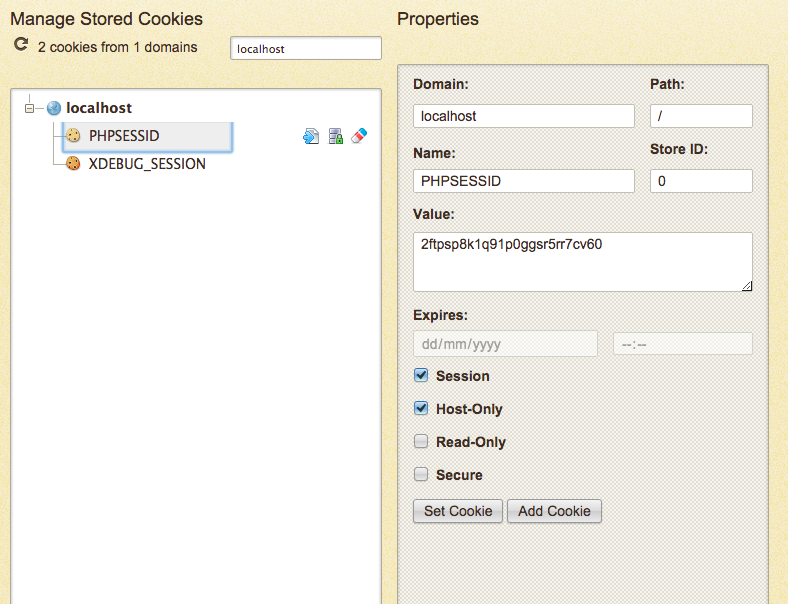
\includegraphics[width=\textwidth]{figures/Doge_Session_Cookie.png}
	\caption{PHPSESSID cookie for the DogeBank application}
\end{figure}


%SESSION 003
\vulntitle{OTG-SESS-003}{Testing for Session Fixation}
\vultable{\doge}{%
	After careful observation and testing we found that once a session ID has been set, this will not be changed until a user logs out. More specifically, the session ID will not be invalidated before a login operation, remaining the same after having logged in (a session ID is generated on the login page already).
}{%
	The session ID generation was thoroughly observed thanks to a Proxy that intercepted all GET/POST requests and responses to/from the server. For this the Burp Suite tool was used.
}{%
	Setting up a possible attack is theoretically easy, but it requires a victim to be tricked by the attacker, making the attack less likely depending on the victim.
}{%
	An attacker could generate a session ID for himself, then force the same ID onto a user, hijacking that users' session in case of successful authentication with the server. This implicates full access to the account of a user.
}{%
	\cvssBaseScorePretty{N}{H}{N}{R}{U}{L}{L}{L}
}
\vultable{\gnb}{%
	Unlike the DogeBank case, the session ID, once generated, never changes. Even though the server destroys all session variables associated to a user, after a logout operation, the session ID is not unset. The session ID is first generated on login page, same as for the DogeBank application.
}{%
	This discovery was made while analyzing the session cookies thanks to the Cookies browser extension.
}{%
	The same likelihood described for the DogeBank application applies.
}{%
	The same implications mentioned for the DogeBank application apply.
}{%
	\cvssBaseScorePretty{N}{H}{N}{R}{U}{L}{L}{L}
}
%SESSION 004
\vulntitle{OTG-SESS-004}{Testing for Exposed Session Variables}
\vultable{\doge}{%
	After observing requests and responses between the client and the server, we observed that session IDs are always sent in HTTP headers. Although the session ID is never explicitly passed in URLs, no encryption is provided whatsoever and the session ID does not change until a user explicitly logs out. No other session variables are generated, therefore only the session ID is affected.
}{%
	This observation was made when analyzing session management. Refer to sections \vulnref{OTG-SESS-001} and \vulnref{OTG-SESS-003}.
}{%
	As long as an attacker can sniff the network traffic and read the session ID of a user, it is very easy to hijack a session. This approach makes it even easier than hijacking a session through social engineering.
}{%
	An attacker can perform a man in the middle attack, read the unencrypted HTTP messages exchanged between a user and the server, in order to impersonate the user and hijack an existing session. This implicates full access to the account of a user.
}{%
	\cvssBaseScorePretty{N}{H}{N}{R}{U}{L}{L}{L}
}
\vultable{\gnb}{%
	The same observations made for the DogeBank application apply.
}{%
	The discovery was made thanks to GET/POST requests interception.
}{%
	The same likelihood described for the DogeBank application applies.
}{%
	The same implications mentioned for the DogeBank application apply.
}{%
	\cvssBaseScorePretty{N}{H}{N}{R}{U}{L}{L}{L}
}
%SESSION 005
\vulntitle{OTG-SESS-005}{Testing for Cross Site Request Forgery}
\vultable{\doge}{%
	Having observed different functionalities offered by the server, we noticed that no encryption is used at all; furthermore the session ID is stored as a cookie in the browser of the user, which makes things a lot easier. In order to trick a user into execute specific operations, however, we found out that some knowledge of the web application was required. Given this knowledge, it proves easy to compromise the entire web application. We found a list of pages potentially subject to CSRF:
	\begin{itemize}
		\item approveuser.php: can be exploited without privileges
		\item approvetransaction.php: can be exploited without privileges
		\item downloadTans.php: can be exploited without privileges
		\item register\_employee.php: only accessible to employees. The existence of this page has to be known to an attacker beforehand
		\item tran.php: although this page is easy to exploit, an attacker would need to have access to the TANs of a user. This could be done beforehand by downloading from \url{/downloadTans.php}
	\end{itemize}
}{%
	All of the observations were made while navigating the website and brute-forcing different combinations of attacks. Other helpful tools helpful were DirBuster and the DogeBankHack custom script, since these allowed to gain a better understanding of the website's structure.
}{%
	In theory, performing a CSRF attack would be easy, since session IDs are stored in browsers and sent over unencrypted channels. However, in this specific case, the attack complexity increases, since the attacker requires additional knowledge, like the ID of a user and the names of the vulnerable pages. In most of the above mentioned cases, getting access to the ID of a user proves to be trivial, since it is contained in pages shown to the user (easy to exploit via Javascript).
}{%
	An attacker in possession of the previously described information could be able to trick a victim into executing operations predetermined by the attacker himself, like starting transactions to arbitrary accounts or registering arbitrary employees. The impact in the former case would compromise the whole bank account of a user, or grant a privilege escalation in the latter case.
}{%
	\cvssBaseScorePretty{N}{H}{N}{R}{U}{L}{H}{L}
}
\vultable{\gnb}{%
	The same predisposition showed by the DogeBank application holds true, i.e. no encryption is used in client-server message exchanges and the session ID is stored as a cookie in the browser of the user. Similar observations regarding the knowledge required to perform a CSRF attack also hold. In particular, these pages proved to be vulnerable:
	\begin{itemize}
		\item verify\_transaction.php: as for the DogeBank case, an attacker would need to have access to the TANs of a user in order to exploit this page. Getting access to these TANs, however, is only possible by either accessing the database directly or intercepting the confirmation email sent to a user;
		\item manage\_registration.php: requires knowledge of the ID of the user that we want to approve/reject. Other than that, exploiting this page proved to be trivial and just required a proper analysis of the client-side code;
		\item manage\_transfer.php: this page is also easy to exploit, since it only requires knowledge of the pending transactions IDs, which can be found on the same page;
		\item manage\_clients.php: although this page can be accessed directly, its existence has to be known to the attacker.
	\end{itemize}
	It is important to stress that, given the layout of the pages, the above mentioned pages can simply be used as section parameters inside a POST request to the employee.php and client.php pages, without the need to copy additional Javascript from the container pages.
}{%
	These observations were made while navigating the website and brute-forcing different combinations of attacks.
}{%
	As for the DogeBank case, although a CSRF attack would be easy, the complexity increases in this specific case, since an attacker needs some knowledge about the layout of the pages (i.e. the names of the above mentioned vulnerable php sections). This information is harder to acquire than in the previous case however, as it required a thorough client-side code analysis.
}{%
	Assuming an attacker is capable of obtaining the required information for such an attack to work, this would have the same implications described in the DogeBank case.
}{%
	\cvssBaseScorePretty{N}{H}{N}{R}{U}{L}{L}{L}
}
%SESSION 006
\vulntitle{OTG-SESS-006}{Testing for logout functionality}
\vultable{\doge}{%
	We observed that the logout functionality is working properly, as the logoutAction.php destroys an existing session, creating a new one. Trying to access a page that requires authentication, after having logged out, fails and the server responds with a "PHPSESSID=deleted" cookie, redirecting the browser to the login page.
	We also observed that there is no logout timer, allowing a user to be logged in indefinitely, as long as the logout is not manually triggered.
}{%
	These observations were made using the Burp Repeater tool.
}{%
	\na
}{%
	Since there is no session timeout policy whatsoever, this could prove to be a vulnerability. This is analyzed in more details in \vulnref{OTG-SESS-007}.
}{%
	\secure
}
\vultable{\gnb}{%
	The same observations made for the DogeBank application apply. Additionally, we found out that the logout functionality does not create a new session ID for the user, but rather destroys all of the server-side variables associated to that user only.
}{%
	These observations were made using the Burp Repeater tool.
}{%
	\na
}{%
	The same implications described for the DogeBank application apply.
}{%
	\secure
}
%SESSION 007
\vulntitle{OTG-SESS-007}{Test Session Timeout}
\vultable{\doge}{%
	We observed that no session timeout policy was implemented, neither on server side nor on client side. Although the only sensitive information stored on client side is the session ID, we proved that it was possible to reuse the same session any number of times.
}{%
	These observations were made using the Burp Repeater tool.
}{%
	A session hijacking is easy to perform, as long as the attacker can either sniff the traffic between the victim and the server, or has access to the device from which the victim logged in.
}{%
	The lack of a session timeout gives a potential attacker indefinite time to perform a session hijacking. Once a session has been hijacked, an attacker has complete access over a user's account.
}{%
	\cvssBaseScorePretty{N}{H}{N}{N}{U}{L}{L}{L}
}
\vultable{\gnb}{%
	The same observations made for the DogeBank application apply.
}{%
	These observations were made using the Burp Repeater tool.
}{%
	The same likelihood described for the DogeBank application applies.
}{%
	The same implications mentioned for the DogeBank application apply.
}{%
	\cvssBaseScorePretty{N}{H}{N}{N}{U}{L}{L}{L}
}
%SESSION 008
\vulntitle{OTG-SESS-008}{Testing for Session puzzling}
\vultable{\doge}{%
	Considering that the only session variable set by the application is the session ID, which we observed is randomly generated by the server, there isn't really any margin for session variable overloading.
}{%
	These observations were made using the Burp suite tool.
}{%
	\na
}{%
	\na
}{%
	\secure
}
\vultable{\gnb}{%
	The same observations made for the DogeBank application apply.
}{%
	These observations were made using the Burp suite tool.
}{%
	\na
}{%
	\na
}{%
	\secure
}

\clearpage
\section{Data Validation Testing}
%\simpleVulntitle{OTG-INPVAL-001}{Testing for Reflected Cross Site Scripting}
\simpleVulntitle{OTG-INPVAL-002}{Testing for Stored Cross Site Scripting}
\vultable{\doge}{%
	All pages showing user defined input are vulnerable to stored cross site scripting.
	No input is validated after it is entered by the user as described in \vulnref{OTG-BUSLOGIC-001}.
}{%
	Issues on multiple pages were discovered during manual testing of the input vectors. For example:
	\begin{itemize}
		\item Site: \texttt{/register.php}
		\item Fields: \texttt{First Name} \texttt{Last Name}
		\item Input example: \texttt{<script>alert(1);</script>}
		\item Shown on:
		\begin{itemize}
			\item \texttt{/customer\_home.php}
			\item \texttt{/tran.php}
			\item \texttt{/employee\_home.php}
		\end{itemize}
	\end{itemize}
	Javascript code can be written to the database using forms. It will later on be automatically executed on client side (e.g.\ comments in transactions)
}{%
	Really easy to perform
}{%
	Total control over the affected sites
}{%
	\cvssBaseScorePretty{N}{L}{N}{N}{U}{H}{H}{H}
}
\vultable{\gnb}{%
	All pages showing user defined input are vulnerable to stored cross site scripting.
	No input is validated after it is entered by the user as described in \vulnref{OTG-BUSLOGIC-001}.
}{%
	Issues on multiple pages were discovered during manual testing of the input vectors. For example:
	\begin{itemize}
		\item Site: \texttt{/registration.php}
		\item Fields: \texttt{First Name} \texttt{Last Name}
		\item Input example: \texttt{<script>alert(1);</script>}
		\item Shown on:
		\begin{itemize}
			\item \texttt{/employee/employee.php} in the manage\_registration section
			\item \texttt{/client/client.php}
		\end{itemize}
	\end{itemize}
}{%
	\same
}{%
	\same
}{%
	\cvssBaseScorePretty{N}{L}{N}{N}{U}{H}{H}{H}
}

%\vulntitle{OTG-INPVAL-003}{Testing for HTTP Verb Tampering}
%\vulntitle{OTG-INPVAL-004}{Testing for HTTP Parameter pollution}

\vulntitle{OTG-INPVAL-005}{Testing for SQL Injection}
\vultable{\doge}{%
	We observed several effective SQL Injection vulnerabilities in the \doge{} site.
	
	The following could be accomplished:
	\begin{itemize}
	
	\item Timing attacks, e.g. using \texttt{username=miWm' AND (SELECT * FROM (SELECT(SLEEP(5)))lqlT)\#}
	\item Logging in without valid user credentials, e.g. using \texttt{username=-6505' OR 7530=7530-- -}	
	
	\end{itemize}
	
}{%
	This was observed using the tool sqlmap and by manual trial and error.
}{%
	This has a high likelihood as this is covered by almost all simple tools for penetration testing and can be easily done by hand.
}{%
	You can log in as the first user in the database without valid login credentials.
}{%
	\cvssBaseScorePretty{N}{L}{N}{N}{U}{H}{H}{H}
}
\vultable{\gnb}{%
	We observed several effective SQL Injection vulnerabilities in the \gnb{} site.
	
	The following could be accomplished:
	\begin{itemize}
	
	\item Timing attacks, e.g. using \texttt{username=miWm' AND (SELECT * FROM (SELECT(SLEEP(5)))lqlT)\#}
	
	\end{itemize}
}{%
	\same
}{%
	\same
}{%
	This allows to send commands to the SQL database and retrieve some information, but not to log in the user.
}{%
	\cvssBaseScorePretty{N}{L}{N}{N}{U}{H}{H}{H}
}

%\vulntitle{OTG-INPVAL-006}{Testing for LDAP Injection}
%\vulntitle{OTG-INPVAL-007}{Testing for ORM Injection}
%\vulntitle{OTG-INPVAL-008}{Testing for XML Injection}
%\vulntitle{OTG-INPVAL-009}{Testing for SSI Injection}
%\vulntitle{OTG-INPVAL-010}{Testing for XPath Injection}
%\vulntitle{OTG-INPVAL-011}{IMAP/SMTP Injection}

\vulntitle{OTG-INPVAL-012}{Testing for Code Injection}
\vultable{\doge}{%
	This vulnerability is not applicable due to the fact that none of the pages of the \doge{} allows to provide a parameter that will be executed. See \vulnref{OTG-INPVAL-013} for a similiar attack using the filename of the uploaded batch transactions file.
}{%
	This was observed using a Proxy that intercepted all GET/POST requests and responses to/from the server. For this the Burp Suite tool was used.
}{%
	\na
}{%
	\na
}{%
	\naScore
}
\vultable{\gnb}{%
	This vulnerability is not applicable due to the fact that none of the pages of the \gnb{} allows to provide a parameter that will be executed.
}{%
	This was observed using a Proxy that intercepted all GET/POST requests and responses to/from the server. For this the Burp Suite tool was used.
}{%
	\na
}{%
	\na
}{%
	\naScore
}

\vulntitle{OTG-INPVAL-012-1}{Testing for Local File Inclusion}
\vultable{\doge}{%
	This vulnerability is not applicable due to the fact that none of the pages of the \doge{} allows to provide a parameter specifying files.
}{%
	This was observed using a Proxy that intercepted all GET/POST requests and responses to/from the server. For this the Burp Suite tool was used.
}{%
	\na
}{%
	\na
}{%
	\naScore
}
\vultable{\gnb}{%
	This vulnerability is not applicable due to the fact that none of the pages of \gnb{} allows to provide a parameter specifying files. The \gnb{} can be exploited though by messing with the internal lookup that gets the php filename from a keyword. See \vulnref{OTG-AUTHZ-001} for a more detailed description.
}{%
	This was observed using a Proxy that intercepted all GET/POST requests and responses to/from the server. For this the Burp Suite tool was used.
}{%
	\na
}{%
	\na
}{%
	\naScore
}

%\vulntitle{OTG-INPVAL-012-2}{Testing for Remote File Inclusion}
\vulntitle{OTG-INPVAL-013}{Testing for Command Injection}
\vultable{\doge}{%
	We found that this vulnerability was strictly related to \vulnref{ORG-BUSLOGIC-009}, since we managed to exploit this vulnerability inside the \texttt{tran.php} page, when uploading a batch transaction file. We observed that it was possible to make the server execute arbitrary commands by injecting them inside the filename of the batch file. The results from stdout were also clearly visible inside the \texttt{tran.php} page.
}{%
	In order to execute arbitrary commands we had to insert them in the name of the uploaded file. Here is an example:\newline
	;cat /etc/passwd;\#\newline
	The content of the file were not really relevant, since we just wanted to execute code on the machine.
}{%
	The likelihood of an attacker attempting a command injection through a file upload is very high.
}{%
	This vulnerability proves as really severe, since an attacker can execute arbitrary commands on the webserver. The results are not too devastating, as long as the attacker does not have access to the root user; however all the source code is visible this way, which can aid the attacker in attempting to exploit further vulnerabilities.
}{%
	\cvssBaseScorePretty{N}{L}{L}{N}{C}{H}{H}{H}
}
\vultable{\gnb}{%
	Similarly to the case of the DogeBank application, we observed that on the new\_transaction\_multiple.php page it was indeed possible to inject commands by inserting them directly into the filename of the file that was to be uploaded.
}{%
	In comparison to the DogeBank case, we had to append the commands after an apostrophe, since the call to the C parser would take parameters inside apostrophes. We also had to camouflage the file itself as a .txt/.csv file, since the web application performs checks on the file extension.
	Here is an example of the filename use for a successful attack:\newline
	hack';cd ..;ls -la;\#.txt\newline	
}{%
	The likelihood of an attacker attempting a command injection through a file upload is very high.
}{%
	The same implications mentioned for the DogeBank case apply. However, since in this case an attacker could have gotten root access (refer to \vulnref{OTG-CONFIG-001}), the implications are much worse.
}{%
	\cvssBaseScorePretty{N}{H}{L}{N}{C}{H}{H}{H}
}
%INPVAL 014
\vulntitle{OTG-INPVAL-014}{Testing for Buffer overflow}
\vultable{\doge}{%
	While testing the DogeBank application for C vulnerabilities, we found the actual code to be difficult to exploit, as inserting any kind of value inside the transaction file tags would not result in segmentation fault or other visible errors. In order to produce overflows and break the program, we had exploit the filename vulnerability, as it allowed us to pass in custom parameters to the C program. It is also important to stress that the batch transaction functionality offers a transaction log, which is displayed on client side after a request and proved to be the direct output of the C parser. This, however, includes by default only stdout messages and not stderr messages. To bypass this, we had to tamper with the transaction filename, in order to redirect stderr messages on stdout and get some feedback.\newline
	More detailed observations about the found vulnerabilities are presented inside the following sections: \vulnref{OTG-INPVAL-014-2}, \vulnref{OTG-INPVAL-014-3} and \vulnref{OTG-INPVAL-014-4}.
}{%
	Finding out these vulnerabilities required multiple attempts. In order to find these vulnerabilities we performed manual attacks and used the Fuzz functionality of the Zed Attack Proxy tool.
}{%
	The complexity of these attacks proved to be much higher than any other while stress-testing this application. Since we were doing Black-box testing, we had to come up with possible combinations of strings in order to find weaknesses inside the C code. Hence an attacker could find vulnerabilities through brute-force, which makes an attack less likely.
}{%
	\na
}{%
	\naScore
}
\vultable{\gnb}{%
	The C Parser seems to be robust, as e did not find any buffer overflow vulnerability, neither due to bad string formats nor due to stack/heap overflow.
}{%	?
	We tried several combinations of brute force attacks, both manually and using the Fuzz functionality of the Zed Attack Proxy tool. We even tried SQL injection inside the fields of the transaction file, with no success.
}{%
	\na
}{%
	\na
}{%
	\secure
}
\vulntitle{OTG-INPVAL-014-2}{Testing for Stack overflow}
\vultable{\doge}{%
	We observed that it was possible to produce stack overflows by tampering with the filenames and calling the C program using custom arguments. This way we were able to generate two different kinds of messages: the program either crashed before starting the correct execution (segmentation fault) or produced a stack smashing error at some point during the transaction processing. Although in both cases a stack overflow is generated, it definitely happens in a different part of the code, since the error messages are different.
}{%
	We discovered this issue by brute-forcing arbitrary values inside the filename. More specifically, we found out that the C program would take in other arguments besides the filename (user/account id most likely). Being this parameter of fixed size, we managed to inject longer values, which could result into stack smashing.
	Here are two examples of filenames that generated two different errors (probably due to difference in length):
	\begin{itemize}
		\item \texttt{testinput.txt hackhackhackhackhack 2>\&1 \#}
		\item \texttt{textinput.txt '0 UNION ALL SELECT tan6 from tans\_lists' 2>\&1 \#}
	\end{itemize}
}{%
	The attack proved to be rather difficult and exploiting the vulnerability properly also requires some skills.
}{%
	Stack overflows allow an attacker to modify the program flow, for example overwriting return addresses.
}{%
	\cvssBaseScorePretty{N}{H}{L}{N}{C}{H}{H}{H}
}
\begin{figure}[h!tbp]
	\centering
	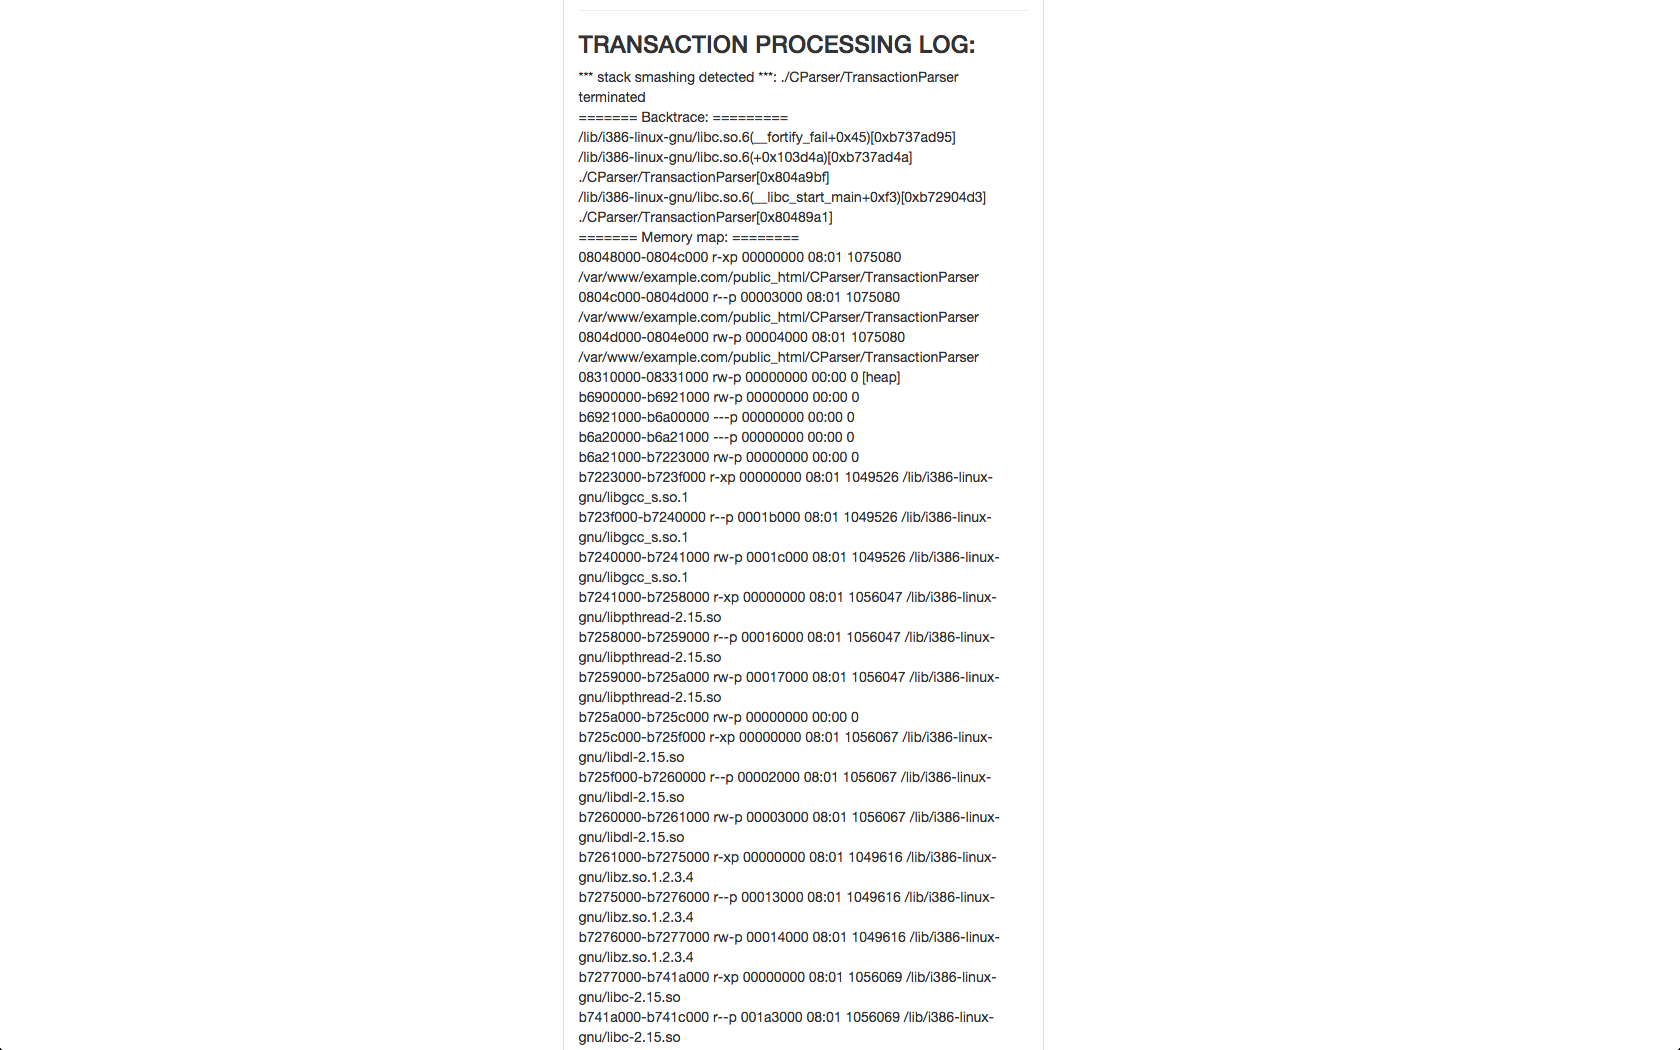
\includegraphics[width=\textwidth]{figures/Doge_C_Stack.png}
	\caption{Stack smashing error generated on the DogeBank \texttt{tran.php} page by uploading the file \texttt{testinput.txt hackhackhackhackhack 2>\&1 \#}}
\end{figure}

\vulntitle{OTG-INPVAL-014-3}{Testing for Heap overflow}
\vultable{\doge}{% 
	Similarly as for the stack overflow, we managed to get a heap overflow by tampering with the filenames and calling the C program using custom arguments. Differently from the stack overfow, we tried using a longer string as a parameter and simultaneously performing SQL injection through it. Although we can't be sure if the SQL injection actually worked, the resulting error was caused by a free() operation. We also noticed that the one filename produced different results in time: \texttt{textinput.txt '0 UNION ALL SELECT tan6 from tans\_lists' 2>\&1 \#} cause both a stack overflow and a heap overflow.
}{%
	Discovery made by fuzzing the values inside the batch transaction file and comparing the results we got back by the server. We also tried several argument strings manually.
}{%
	The attack proved to be rather difficult and exploiting the vulnerability properly also requires some skills.
}{%
	Heap overflows allow an attacker to modify the program flow, leading to arbitrary code execution.
}{%
	\cvssBaseScorePretty{N}{H}{L}{N}{C}{H}{H}{H}
}
\begin{figure}[h!tbp]
	\centering
	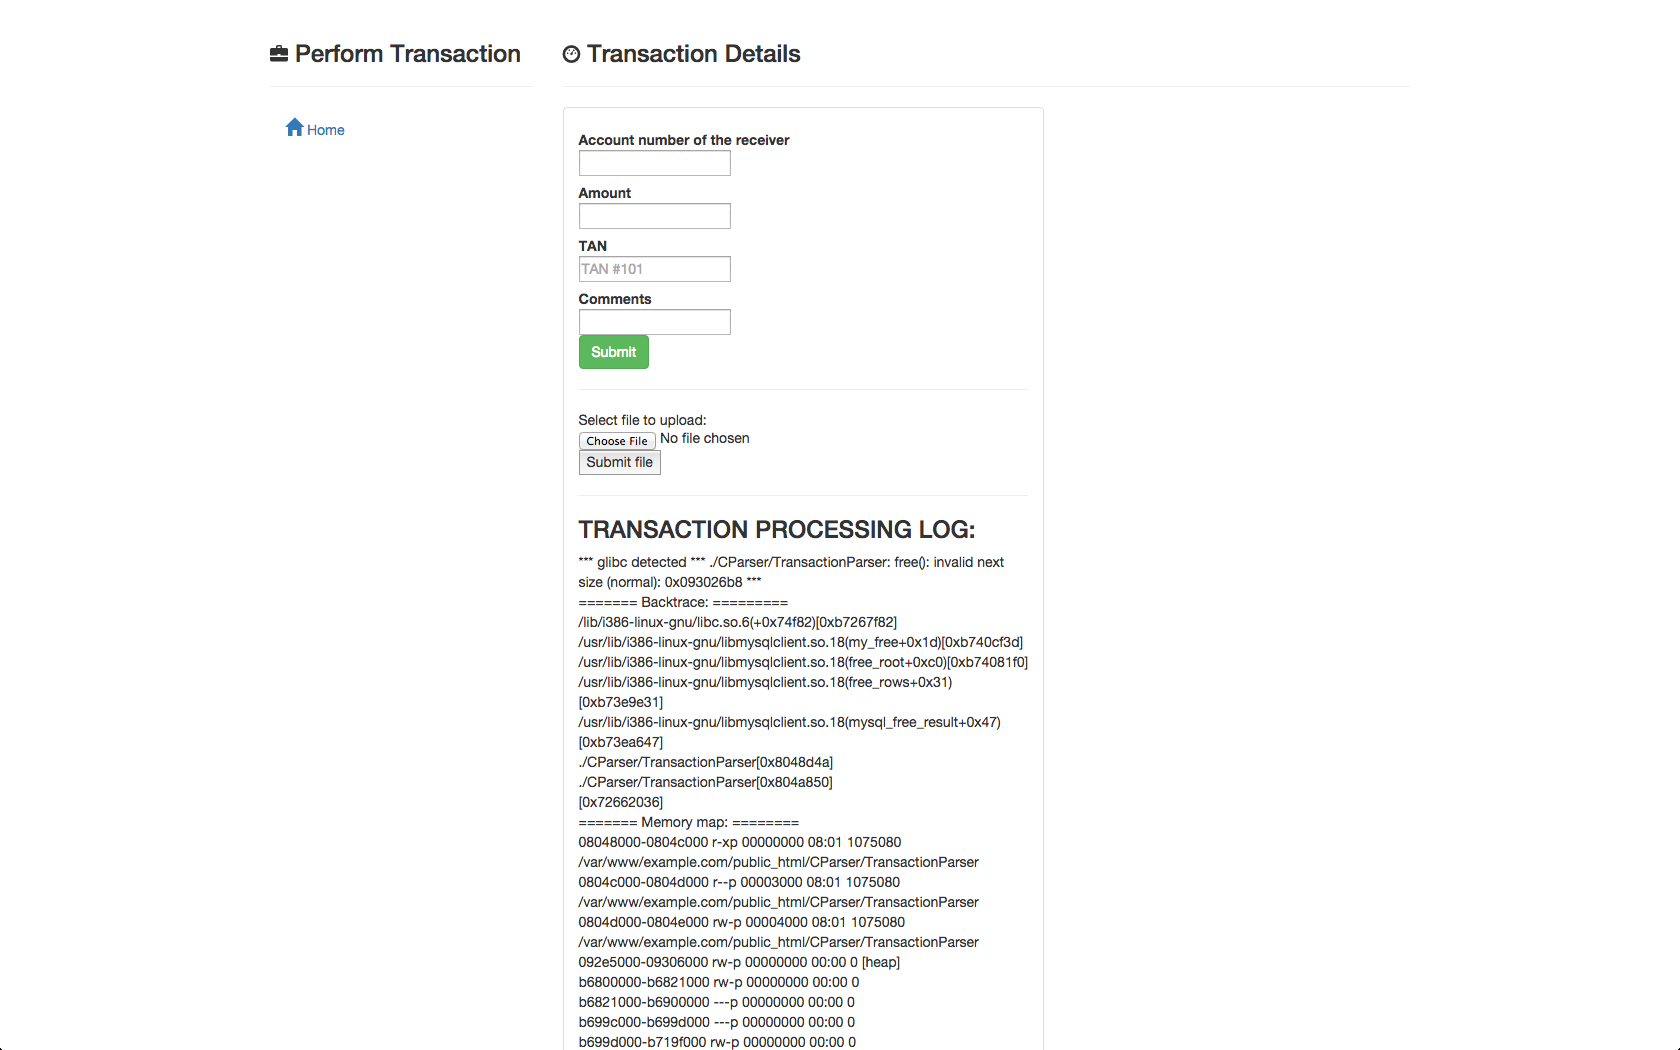
\includegraphics[width=\textwidth]{figures/Doge_C_Heap.png}
	\caption{Heap error generated on the DogeBank \texttt{tran.php} page by uploading the file \texttt{textinput.txt '0 UNION ALL SELECT tan6 from tans\_lists' 2>\&1 \#}}
\end{figure}
\vulntitle{OTG-INPVAL-014-4}{Testing for Format string}
\vultable{\doge}{%
	The only issue we found when working with string formats was regarding to the length of a string. When passed a huge string, the program will simply not work as intended, probably due to buffer limitations. However, no relevant error messages were returned, hence the file is definitely not read using the \textit{gets} function.\newline
	Inserting null characters inside the file also makes the program not work as intended, but it is not possible to exploit the actual transaction functionality by doing this.
}{%
	Most of these discoveries were made by fuzzing the values inside the batch transaction file and comparing the results we got back by the server.
}{%
	This does not prove to be an actual attack, since it doesn't break the C program by allowing to exploit the code.
}{%
	\na
}{%
	\naScore
}

%INPVAL 015
\vulntitle{OTG-INPVAL-015}{Testing for incubated vulnerabilities}
\vultable{\doge}{%
	Since it is possible to upload files permanently onto the webserver and the application is already vulnerable to XSS attacks and SQL injections, incubated attacks are definitely an option.
}{%
	This vulnerability depends on the possibility to store malicious code on the server, hence it is a consequence of discovering other vulnerabilities like the upload of malicious files.
}{%
	The likelihood of such an attack is high, although in some cases social engineering may be required. For example, performing a stored XSS attack during a registration process will result in every employee executing that particular script.
}{%
	Tricking a user into executing malicious code can prove to be a very serious issue.
}{%
	\cvssBaseScorePretty{N}{H}{L}{N}{U}{L}{L}{L}
}
\vultable{\gnb}{%
	The same observations made for the DogeBank application apply.
}{%
	The discovery was made the same way it was for DogeBank case.
}{%
	The same likelihood described for the DogeBank application applies.
}{%
	The same implications mentioned for the DogeBank application apply.
}{%
	\cvssBaseScorePretty{N}{H}{L}{N}{U}{L}{L}{L}
}

\vulntitle{OTG-INPVAL-016}{Testing for HTTP Splitting/Smuggling}
This vulnerability was not tested as we did not extend our testing to the Apache Web Server.

%\clearpage
%\section{Error Handling}
%\simpleVulntitle{OTG-ERR-001}{Analysis of Error Codes}
%\vulntitle{OTG-ERR-002}{Analysis of Stack Traces}

\clearpage
\section{Cryptography}
\simpleVulntitle{OTG-CRYPST-001}{Testing for Weak SSL/TSL Ciphers, Insufficient Transport Layer Protection}
\vultable{\doge}{%
	Due to the fact, that the application is only accessible via HTTP and no SSL/TLS encryption is used no testing for weak ciphers could be performed.
	Relevant information leakage resulting from the unencrypted communication has already been covered in \vulnref{OTG-CONFIG-007} and \vulnref{OTG-CRYPST-003}.
}{%
	\na
}{%
	\na
}{%
	\na
}{%
	\naScore
}
\vultable{\gnb}{%
	The same observations made for the DogeBank application .
	Relevant information leakage resulting from the unencrypted communication has already been covered in \vulnref{OTG-CONFIG-007} and \vulnref{OTG-CRYPST-003}.
}{%
	\na
}{%
	\na
}{%
	\na
}{%
	\naScore
}

\vulntitle{OTG-CRYPST-002}{Testing for Padding Oracle}
\vultable{\doge}{%
	Due to the fact, that no encryption is used when accessing the application, no padding of information is used.
	Relevant information leakage resulting from the unencrypted communication has already been covered in \vulnref{OTG-CONFIG-007} and \vulnref{OTG-CRYPST-003}.
}{%
	\na
}{%
	\na
}{%
	\na
}{%
	\naScore
}
\vultable{\gnb}{%
	The same observations made for the DogeBank application apply.
	Relevant information leakage resulting from the unencrypted communication has already been covered in \vulnref{OTG-CONFIG-007} and \vulnref{OTG-CRYPST-003}.
}{%
	\na
}{%
	\na
}{%
	\na
}{%
	\naScore
}

\vulntitle{OTG-CRYPST-003}{Testing for Sensitive information sent via unencrypted channels}
\vultable{\doge}{%
	Sensitive information is sent over unencrypted channels in every request the user performs as the application is only accessible via HTTP and no SSL/TLS encryption is used.
}{%
	As documented in \vulnref{OTG-CONFIG-007}, the site is not available via HTTPS.
}{%
	Every requests gets sent over an unencrypted channel automatically.
}{%
	The same implications as in \vulnref{OTG-CONFIG-007} apply.
	By sniffing the network traffic, all data exchanged between the server and the client can be read as clear text. No confidentiality at all is supported on this end.
}{%
	\cvssBaseScorePretty{N}{H}{N}{R}{U}{H}{H}{N}
}
\vultable{\gnb}{%
	\same
}{%
	\same
}{%
	\same
}{%
	\same
}{%
	\cvssBaseScorePretty{N}{H}{N}{R}{U}{H}{H}{N}
}

\clearpage
\section{Business Logic Testing}
\simpleVulntitle{OTG-BUSLOGIC-001}{Test Business Logic Data Validation}
\vultable{\doge}{%
	We observed several flaws in the input validation on the \doge{} site. This includes the following fields from a business logic perspective:
	
	\begin{itemize}
	
	\item Transaction Destination Account number \hfill \newline
	This field is not validated. This means money can be transferred to any given account, even if it does not exist. This also enables transferring money to the same account it is coming from. This would not be an issue if this worked properly - but the amount does not get deducted from the source account in this case. Any user may generate infinite money this way.
	
	\item Transaction Amount \hfill \newline
	This field is not validated. This means the transaction amount can even be negative, leading to the specified amount being subtracted from the destination account. This enables "stealing" money from other people's accounts.

	\item Transaction Number \hfill \newline
	This field is not validated. The TAN is not checked for its format which always leads to a check for the given TAN in the database. In combination with the issue that there are no new TANs generated once the 100 given ones are used this leads to the strange vulnerability that the 101st transaction and all following ones do not need a TAN in order to succeed. This means that all transactions accept an empty TAN once all 100 TANs are used.
	
	\end{itemize}
	
	There furthermore is an issue with the logic behind the approval of transactions: Transactions with an amount above 10.000 EUR are only deducted once they are approved. This means it is possible to create additional transactions during the transaction is unapproved, even if the account balance would be negative after the first transaction. Additionally transactions leading to increased negative balance can be done once the account balance is negative.
		
}{%
	Manual testing
}{%
	High
}{%
	This allows an attacker to increase his own account balance without limit and create transactions without the necessary TANs.
}{%
	\cvssBaseScorePretty{N}{L}{L}{N}{U}{N}{H}{L}
}
\vultable{\gnb}{%
	\begin{itemize}
	\item Transaction Destination Account number \hfill \newline
	This field is not validated. This means money can be transferred to any given account, even if it does not exist. This also enables transferring money to the same account it is coming from. This would not be an issue if this worked properly - but the amount does not get deducted from the source account in this case. Any user may generate infinite money this way.
	\end{itemize}
}{%
	Manual testing
}{%
	High
}{%
	This allows an attacker to increase his own account balance without limit.
}{%
	\cvssBaseScorePretty{N}{L}{L}{N}{U}{N}{H}{N}
}

%\vulntitle{OTG-BUSLOGIC-002}{Test Ability to Forge Requests}
%\vulntitle{OTG-BUSLOGIC-003}{Test Integrity Checks}

\vulntitle{OTG-BUSLOGIC-004}{Test for Process Timing}
\vultable{\doge}{%
	We did not observe any process timing vulnerabilities at the \doge{}.
}{%
	We used a custom script to test the response time given invalid and valid usernames and calculated the median response time.
}{%
	\na
}{%
	\na
}{%
	\secure
}
\vultable{\gnb}{%
	We observed a timing attack at the \gnb{}. The response times differ depending on the existence of the provided mail address in the database.
}{%
	\same
}{%
	\na
}{%
	\na
}{%
	\cvssBaseScorePretty{N}{L}{N}{N}{U}{L}{N}{N}
}

%\vulntitle{OTG-BUSLOGIC-005}{Test Number of Times a Function Can be Used Limits}
%\vulntitle{OTG-BUSLOGIC-006}{Testing for the Circumvention of Work Flows}

\vulntitle{OTG-BUSLOGIC-007}{Test Defenses Against Application Mis-use}
\vultable{\doge}{%
	After thorough testing and observation we concluded that no mechanisms to prevent against application mis-use are in place. No critical functionalities are disabled and no logs are kept.
}{%
	These observations were made after using several different tools and manually stress-testing the application.
}{%
	\na
}{%
	This vulnerability implicates that an attacker will be able to attempt countless attacks and abuse functionalities without any repercussion.
}{%
	\cvssBaseScorePretty{N}{L}{N}{N}{U}{L}{L}{L}
}
\vultable{\gnb}{%
	The same observations made for the DogeBank application apply.
}{%
	These observations were made after using several different tools and manually stress-testing the application.
}{%
	\na
}{%
	The same implications mentioned for the Doge application apply.
}{%
	\cvssBaseScorePretty{N}{L}{N}{N}{U}{L}{L}{L}
}

\vulntitle{OTG-BUSLOGIC-008}{Test Upload of Unexpected File Types}
\vultable{\doge}{%
	We discovered that the tran.php page allows to upload any kind of file, without performing extension checks on it. However, it seems that the server accepts only files with a limited size, making it impossible to generate more than 3 transactions at once, or uploading huge files for that matter. Regardless, as long as the filesize stays below 500 bytes, any file will be accepted by the server and stored forever inside the /uploads folder.
}{%
	It is important to stress that no file format was described on the documentation nor on the transaction page. Nonetheless, after having found out the structure of the web application (using DirBuster and Burp), we found a sample batch transaction file in txt format. Afterwards we simply tried uploading files with different extensions to see the outcome.
}{%
	The likelihood of a an attacker uploading a file with a bad filename or a non-expected extension is very high.
}{%
	This was by far the most severe vulnerability we found, since all uploaded files are kept inside a well known folder on the web server. An attacker is this way able to upload any file, as well as custom scripts and programs to the server. This issue is analyzed in depth in section 009.
}{%
	\cvssBaseScorePretty{N}{L}{L}{N}{C}{H}{H}{H}
}
\vultable{\gnb}{%
	The only page which allows to upload a file to the server is the new\_transaction\_multiple.php (loaded as a frame under the my\_accounts.php section inside the client.php file). When uploading a file, the server performs an explicit check, eventually accepting only .csv and .txt files.
}{%
	We tried uploading several files with different file extensions, leading to the result described above.
}{%
	\na
}{%
	\na
}{%
	\secure
}

\vulntitle{OTG-BUSLOGIC-009}{Test Upload of Malicious Files}
\vultable{\doge}{%
	Once discovered that the tran.php page allowed to upload any kind of file, we did multiple tests and finally observed that it was indeed possible to upload malicious code. This vulnerability was later on used to execute custom PHP scripts. Although eventually we gained full access to the application, including credentials, database access and source code, we couldn't tamper too much with the operating system since we didn't have root access.
}{%
	This discovery depends directly on the one made in section \vulnref{OTG-BUSLOGIC-008}.
	We tried multiple attacks in order to exploit this vulnerability, all of which worked without flawlessly:
	\begin{itemize}
		\item Upload a php script which allowed us to start a reverse shell attack.
		\item Upload an interactive php script which could allow us to enter commands directly or perform specific operations.
		\item Upload a php script which could make us tamper with the database.
	\end{itemize}
	Once uploaded, each script could simply be executed by opening the page \texttt{/upload/SCRIPTNAME}
}{%
	Once an attacker asserted the possibility of uploading any kind of file, the likelihood of such an attack becomes very high.
}{%
	As stated in the \vulnref{OTG-BUSLOGIC-008} section, this was the most severe vulnerability found, since it allows to get full control over the application.	
}{%
	\cvssBaseScorePretty{N}{L}{L}{N}{C}{H}{H}{H}
}
\vultable{\gnb}{%
	Although the application performs a check on the extension of the file uploaded via the new\_transaction\_multiple.php page, it does not check the content nor the basename of the file. Combined with the fact code injection is possible due to the same vulnerability (discussed in INPVAL 013), we observed that it is perfectly feasible to upload malicious files and rename them afterwards.
}{%
	This discovery was made thanks to manual attempts to perform code injection. More specifically, we could upload a malicious file and execute by following these steps:
	\begin{enumerate}
		\item Upload a file named \texttt{maliciousFile.txt};
		\item Upload a second file named \texttt{test';mv maliciousFile.txt maliciousFile.php;\#.txt}
		\item Knowing that the uploaded files are stored inside the /uploads folder, the maliciousFile could be executed opening the page \texttt{http://HOST/gnb/project/uploads/maliciousFile.php}
	\end{enumerate}
}{%
	The likelihood of an attacker attempting a code injection through a file upload is very high.
}{%
	The implications of a code injection attack are very severe, since an attacker could execute arbitrary code on the webserver. Even reading source code becomes possible.
}{%
	\cvssBaseScorePretty{N}{L}{L}{N}{C}{H}{H}{H}
}
\begin{figure}[h!tbp]
	\centering
	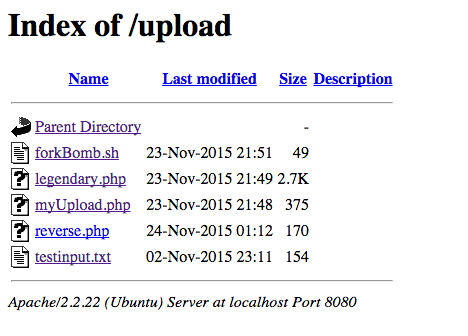
\includegraphics[width=\textwidth]{figures/Doge_Upload.png}
	\caption{List of uploaded files accessible via the \texttt{/upload} folder, after having uploaded some custom scripts}
\end{figure}

\clearpage
\section{Client Side Testing}
This section was prioritized as low, therefore the client side was not tested in depth. Furthermore, as stated in the OWASP testing guide, black box testing of the client side is usually not performed, since access to the source code is always available, as it needs to be sent to the client to be executed.

%\vulntitle{OTG-CLIENT-001}{Testing for DOM based Cross Site Scripting}
%\vulntitle{OTG-CLIENT-002}{Testing for JavaScript Execution}
%\vulntitle{OTG-CLIENT-003}{Testing for HTML Injection}
%\vulntitle{OTG-CLIENT-004}{Testing for Client Side URL Redirect}
%\vulntitle{OTG-CLIENT-005}{Testing for CSS Injection}
%\vulntitle{OTG-CLIENT-006}{Testing for Client Side Resource Manipulation}
%\vulntitle{OTG-CLIENT-007}{Test Cross Origin Resource Sharing}
%\vulntitle{OTG-CLIENT-008}{Testing for Cross Site Flashing}
%CLIENT 009
\vulntitle{OTG-CLIENT-009}{Testing for Clickjacking}
\vultable{\doge}{%
	We observed that it is entirely possible to load all of the pages inside
}{%
	This discovery required manual testing: an html with a simple iframe was included, that could contain any of the pages of the the web application.
}{%
	Considering there is not protection against clickjacking attacks whatsoever, this kind of attack could prove to be quite easy.
}{%
	The Doge web application is entirely vulnerable to clickjacking attacks and an attacker could handle all of the actions started on the php pages in a malicious way.
}{%
	\cvssBaseScorePretty{N}{H}{N}{R}{U}{L}{L}{L}
}
\vultable{\gnb}{%
	The same observations made for the DogeBank application apply.
}{%
	This discovery required manual testing: an html with a simple iframe was included, that could contain any of the pages of the the web application.
}{%
	The same likelihood described for the DogeBank application applies.
}{%
	The GNB web application is entirely vulnerable to clickjacking attacks and an attacker could handle all of the actions started on the php pages in a malicious way.
}{%
	\cvssBaseScorePretty{N}{H}{N}{R}{U}{L}{L}{L}
}

\vulntitle{OTG-CLIENT-010}{Testing WebSockets}
\vultable{\doge}{%
	The Doge Web Application does not make use of any asynchronous operation, neither using AJAX nor using WebSockets.
}{%
	We asserted that there was no WebSockets communication at all while surfing the pages of the application and testing out all of the functionalities. This was done using Google Chrome's Developer Tools.
}{%
	\na
}{%
	\na
}{%
	\secure
}
\vultable{\gnb}{%
	Although the application makes use of asynchronous requests for the client search functionality, this is done using traditional AJAX and not HTML5 WebSockets. Hence, the application is secure against attacks on WebSockets.
}{%
	To prove our observation, we used Google Chrome's Developer Tools to assert there was no ongoing WebSocket communication when executing search requests.
}{%
	\na
}{%
	\na
}{%
	\secure
}

%\vulntitle{OTG-CLIENT-011}{Test Web Messaging}
%\vulntitle{OTG-CLIENT-012}{Test Local Storage}
